\documentclass{article}

\usepackage{graphicx}

\begin{document}

\begin{figure}
  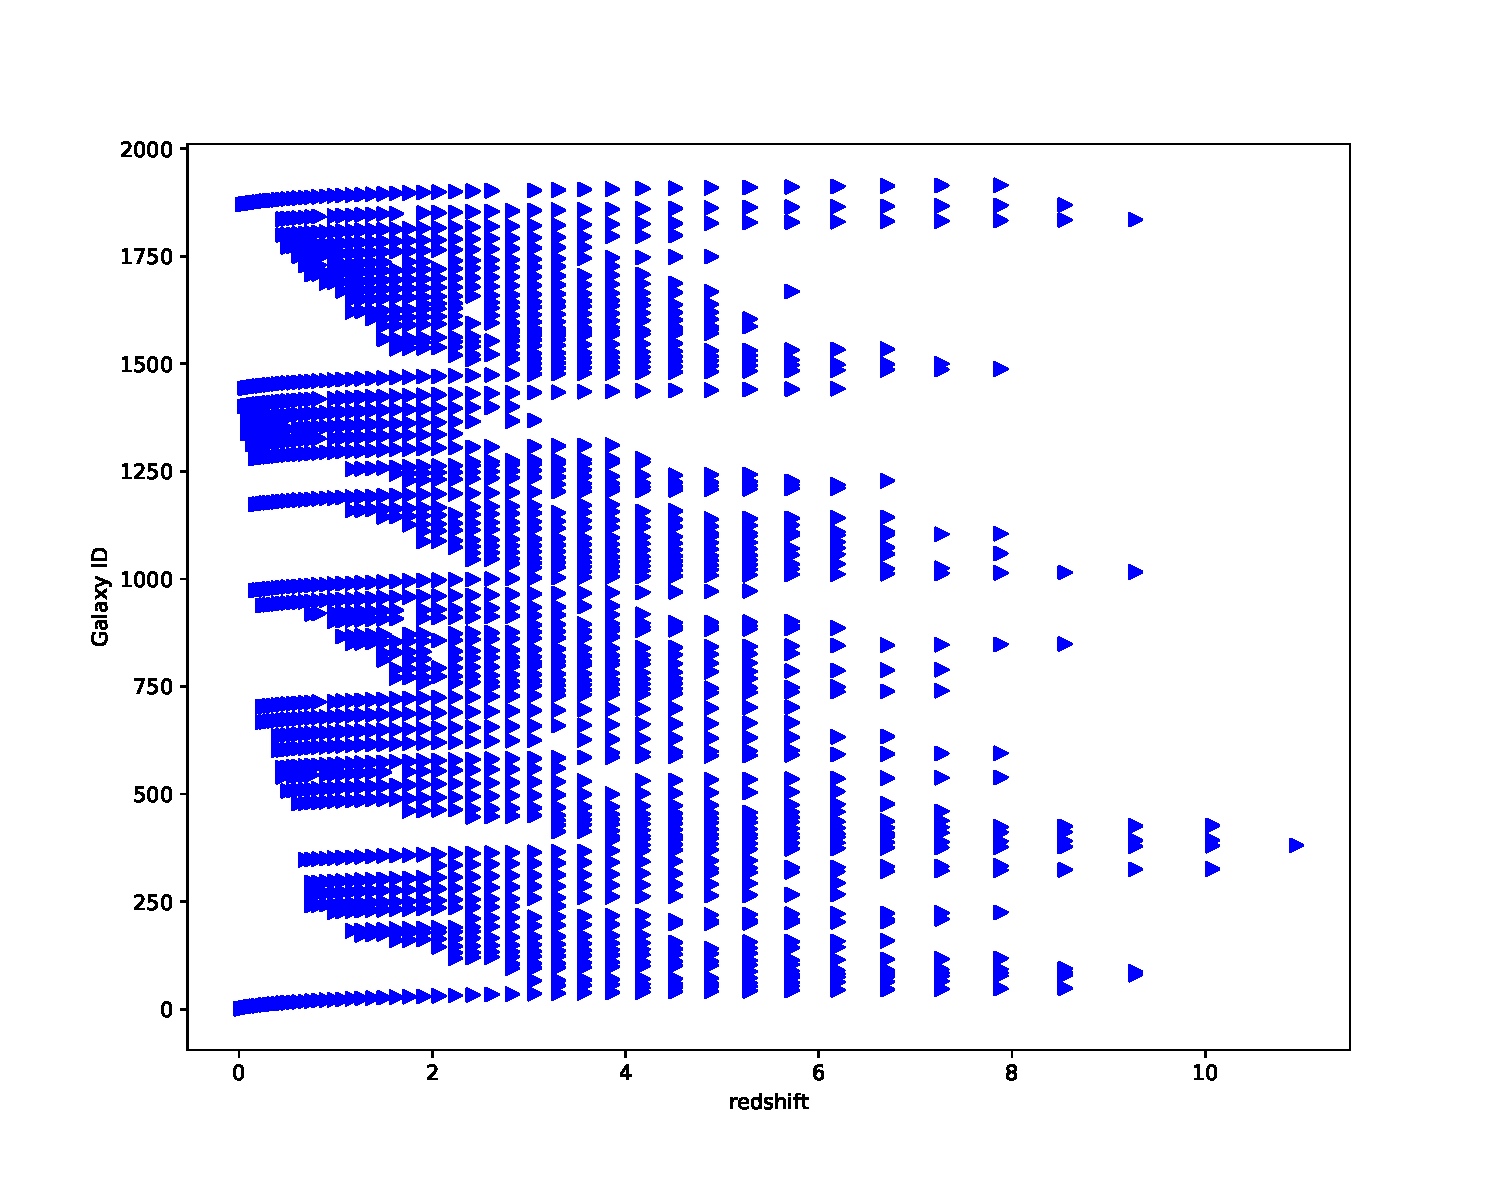
\includegraphics[width=\linewidth]{redshift.pdf}
  \caption{Graph of Galaxy ID versis redshift. This graph illustrates the distribution of different galaxies at a given redshift. This redshift represents the time the light left the galaxy and we use this as a proxy measurement of the galaxy's age.The lack of some IDs at more recent redshifts suggests those galaxies become subsumed by larger ones at prior redshifts.}
  \label{fig:redshift}
\end{figure}

\begin{figure}
  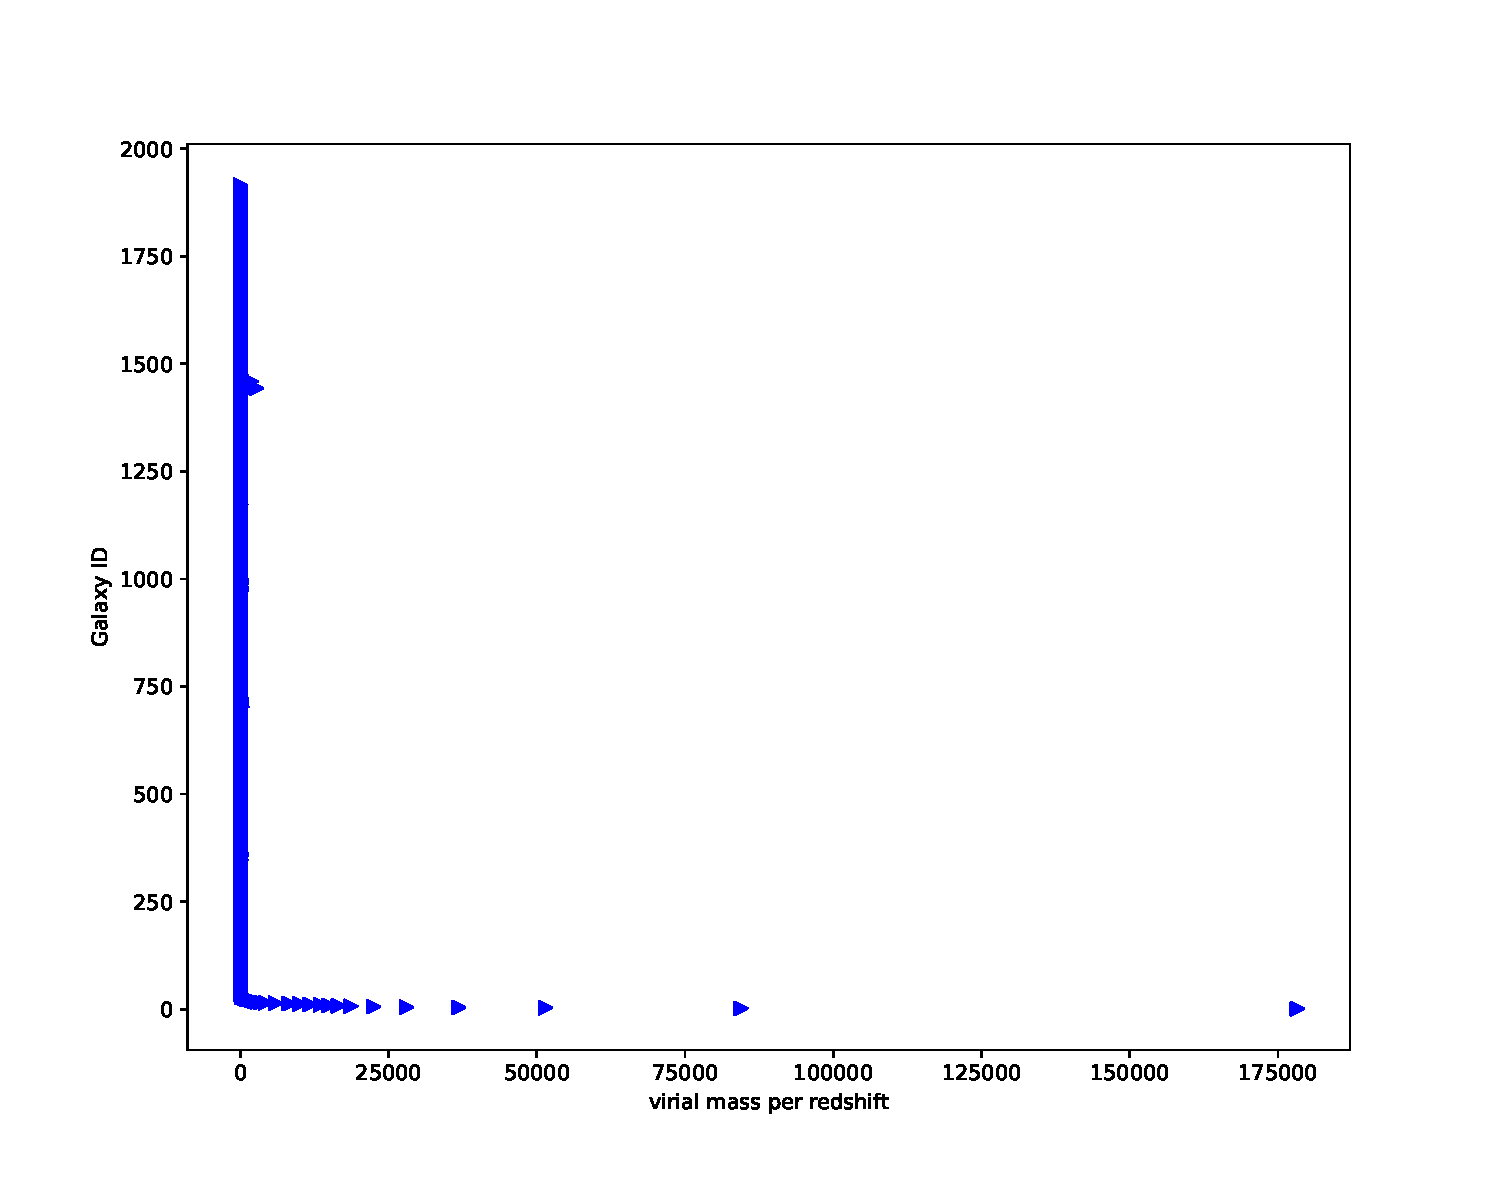
\includegraphics[width=\linewidth]{virial mass per redshift.pdf}
  \caption{Graph of galaxy ID versus virial mass per redshift ($\frac{M_v}{z}$). This graph shows the distribution of virial mass per redshift. A few IDs may have more than one value. This is probably due to change in virial mass over the course of their lifespan.}
  \label{fig:virmass_per_z}
\end{figure}

\begin{figure}
  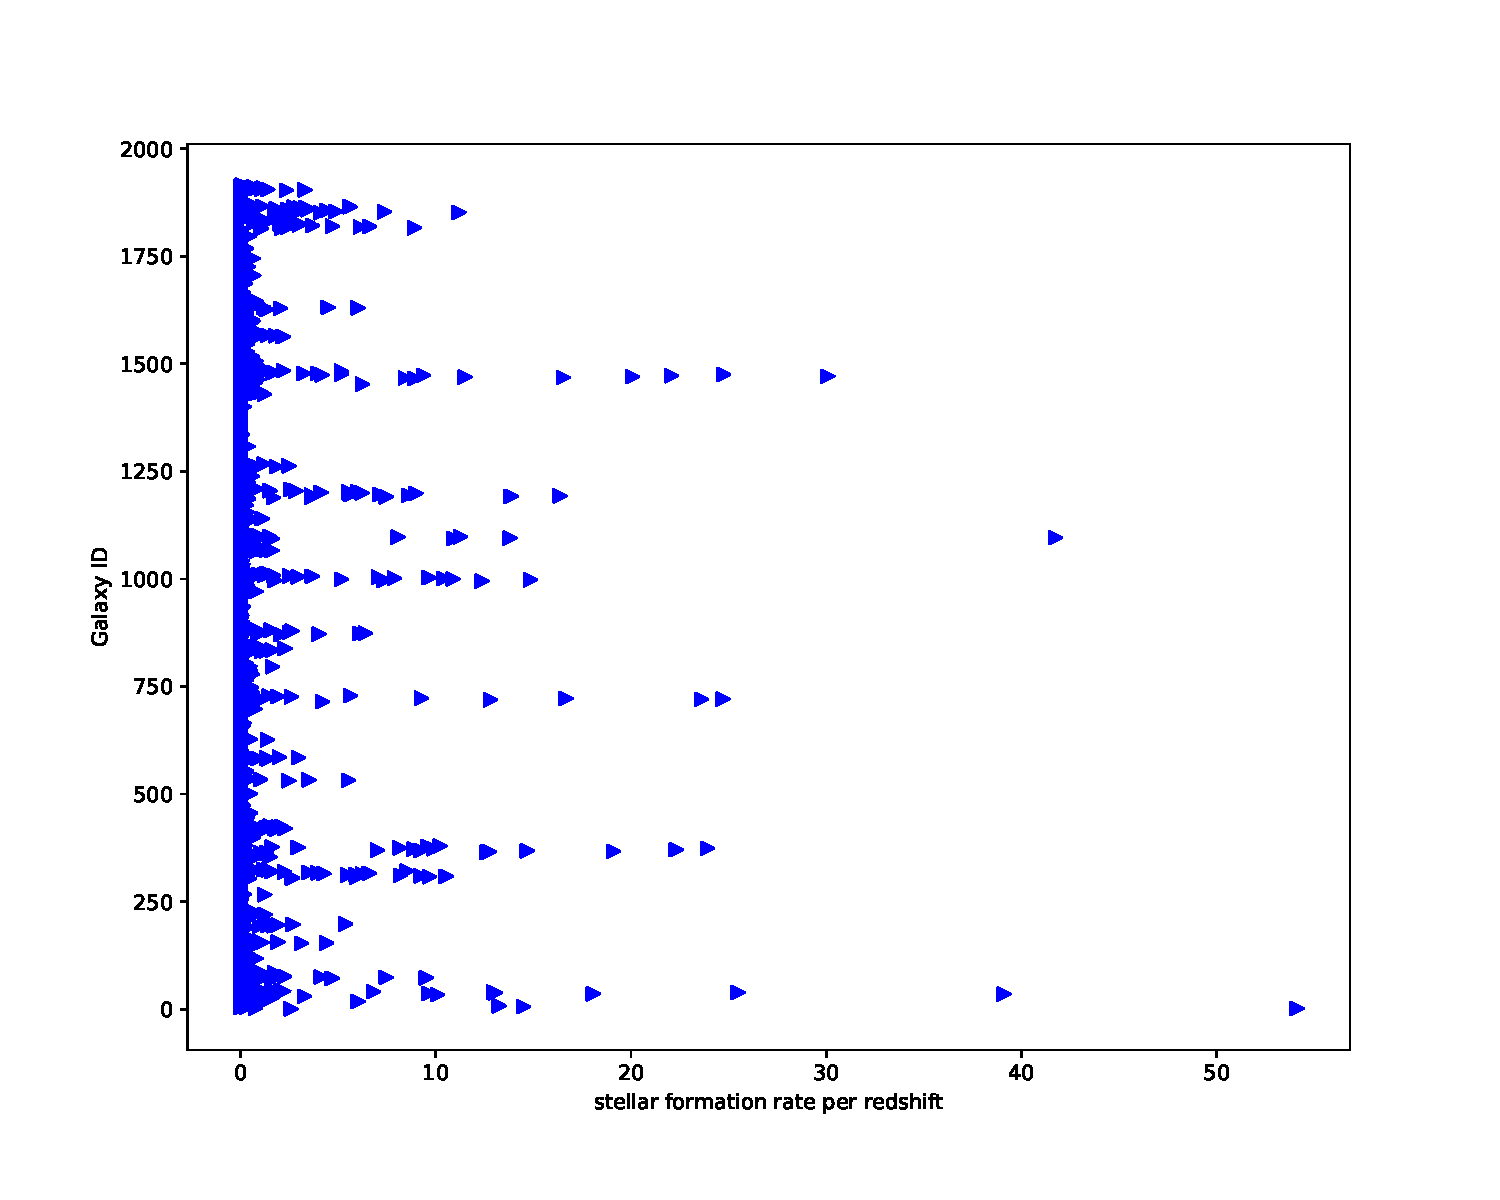
\includegraphics[width=\linewidth]{stellar formation rate per redshift.pdf}
  \caption{Graph of galaxy ID versus stellar formation rate per redshift ($\frac{SFR}{z}$). Many IDs have multiple points. This reflects change in stellar formation rate over the course of their life.}
  \label{fig:sfr_per_z}
\end{figure}

\begin{figure}
  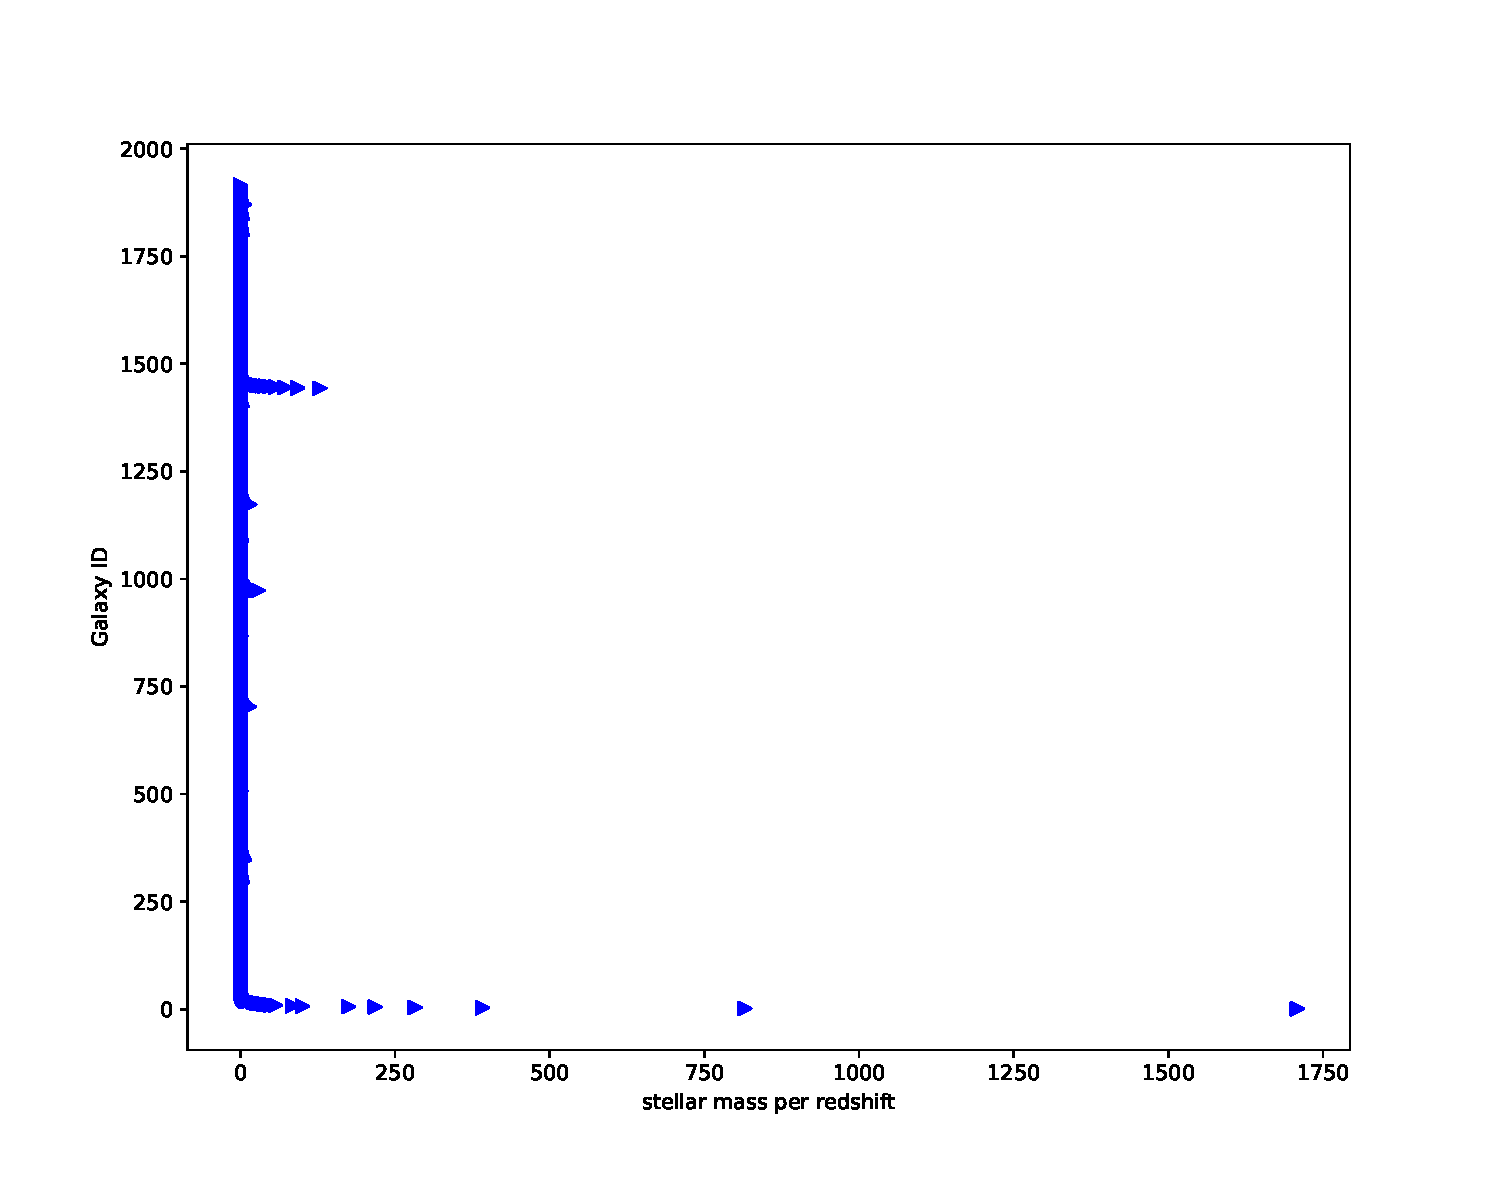
\includegraphics[width=\linewidth]{stellar mass per redshift.pdf}
  \caption{Graph of galaxy ID versus stellar mass per redshift ($\frac{M_*}{z}$). Some IDs have multiple points. This is because it represents the accumulation of living stars and remnants over the course of their life.}
  \label{fig:stellarmass_per_z}
\end{figure}

\begin{figure}
  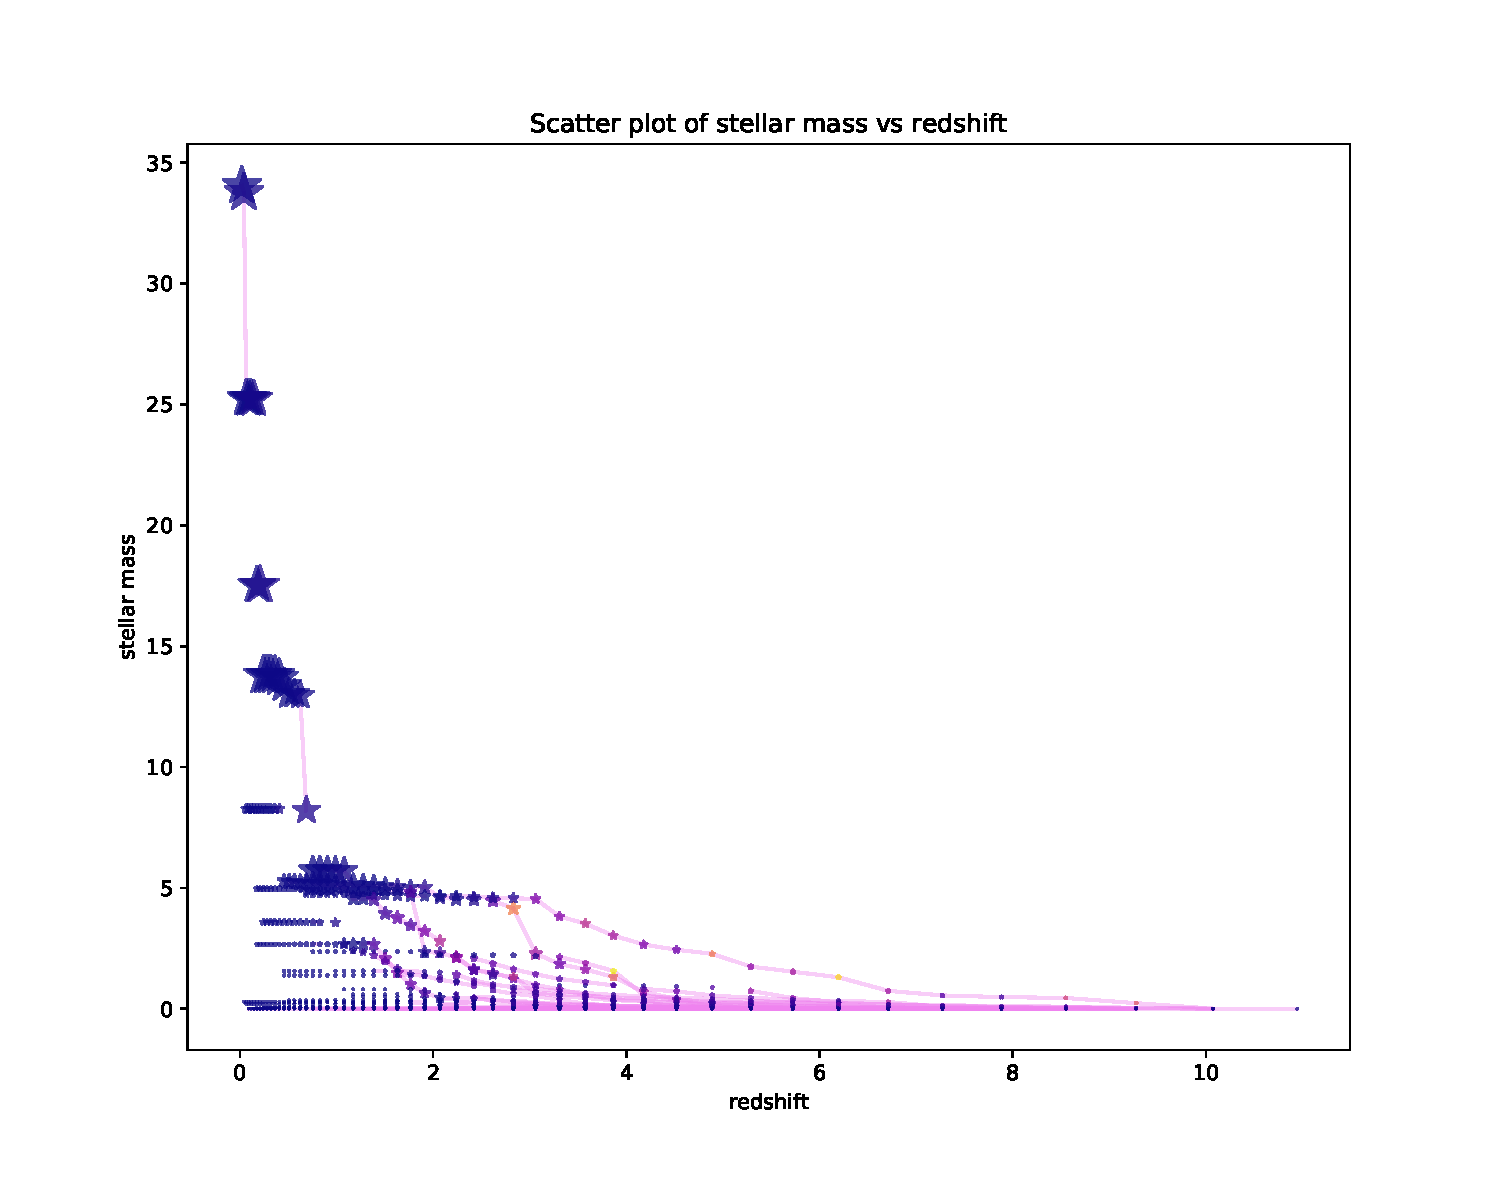
\includegraphics[width=\linewidth]{first merger tree.pdf}
  \caption{scatter plot of stellar mass vs redshift with lines connecting points of increasing virial mass. The colour and size of the dots represent stellar formation rate and virial mass respectively. The overall structure looks like a tree, suggesting a hierarchical means by which the galaxies crash into each other. We define a major merger as a two large galaxies combining. In the above diagram, two large points fusing into an even larger point can be thought to represent a major galaxy merger.}
  \label{fig:first_merger_tree}

\end{figure}

\end{document}
